\documentclass[12pt,titlepage]{article}

% This first part of the file is called the PREAMBLE. It includes
% customizations and command definitions. The preamble is everything
% between \documentclass and \begin{document}.

\usepackage[margin=1in]{geometry}  	% set the margins to 1in on all sides
\usepackage{setspace} \doublespacing 	% double spaced
\usepackage{graphicx}              			% to include figures
\usepackage{subcaption}				% to use sub captions
\usepackage{epstopdf}
\usepackage{amsmath}               		% great math stuff
\usepackage{amsfonts}              		% for blackboard bold, etc
\usepackage{amsthm}                		% better theorem environments
\usepackage[numbers]{natbib}			% for bibiliography with numbers
\usepackage{hyperref}				% make link clickable


%%%%%%%%%%%%%%%%%%%%%%%%
% Document Begins Here %
%%%%%%%%%%%%%%%%%%%%%%%%

\begin{document}

\begin{titlepage}
    \begin{center}
        \vspace*{1cm}


        {\scshape\Large CMPUT681\par}
        {\scshape\LARGE Parallel and Distributed Systems\par}   
        \vspace{0.5cm}
        {\scshape\Large Project Report - Fall 2022\par}
        \vfill
        
        %%%% PROJECT TITLE
        \Huge
        \textbf{The eXpress Data Path\\}
        \LARGE
        Fast Programmable Packet Processing in the Operating System Kernel

        \vfill

        %%%% AUTHOR(S)
        {\Large Naveenraj Muthuraj\par}
        {\Large nmuthura@ualberta.ca \par}
        {\Large 1769237 \par}

    \end{center}
\end{titlepage}

\doublespacing
\tableofcontents
\singlespacing

\newpage

\doublespacing


\section{Introduction}

Network stacks in general purpose operating systems are typically optimised for flexibility. 
This means they perform too many operations per packet, this will eventually lead to bottleneck in network performance  since the network devices and interfaces nowadays come with high speed packets rates upto 100Gbps . This has led to the increasing popularity of software packet processing, such as Data Plane Development Kit (DPDK) \cite{dpdk}. These tools are implemented using kernel bypass techniques, where a userspace application takes complete control of the networking hardware to avoid expensive context switch between kernel and userspace. 

While the kernel bypass approach can significantly improve performance it has its own drawbacks. Firstly, It is difficult to integrate with existing system. Secondly the applications have to re-implement functionality otherwise provided by the operating system network stack, 
such as routing tables and higher level protocols. Lastly, userspace application implementing entire networking stack will increase complexity and blurs security boundaries otherwise enforced by the operating system kernel. 

To overcome these drawbacks of kernel bypass design. \citet{xdp} presented a system that adds programmability directly in the operating system networking stack in a cooperative way. This makes it possible to perform high-speed packet processing that integrates seamlessly with existing systems, while selectively leveraging functionality in the operating system. This framework, called the eXpress Data path (XDP). 

In this report we present a brief introduction to XDP and the results of reproducing the experiments originally conducted by \citet*{xdp}, which shall be referred to has the \textit{original paper} throughout this report.
This is structured as follows: Section 2 brief note on XDP, Section 3 experiment setup and Section 4 presents performance evaluation in comparison to original study and Section 5 Illustrates the use of XDP in real-world use cases and its performance graphs. Section 6 concludes.

\section{The XDP}

eXpress Data Path (XDP) works by defining a limited execution environment in the form of a virtual machine running eBPF code, an extended version of original BSD Packet Filter(BPF) \cite{mccanne_bsd_1993} byte code format.  The BPF environment executes eBPF programs (custom code) in the kernel space, before the kernel itself touches the packet data. Hence allowing packet processing at the earliest possible point after a packet is received from the network interface. The safety of the custom eBPF code is guaranteed  by The eBPF verifier. 

XDP which first got merged into the Linux kernel at version 4.8 , has since been actively developed and adopted across the industries. To name a few, Cloudflare uses XDP for their Distributed Denial of Service (DDoS) Mitigation \cite{cloudflare-ddos} and Facebook uses XDP in their Katran \cite{katran} project which is used for  Layer 4 Load-Balancing at scale. The vast applications of eXpress Data Path (XDP) and the eBPF virtual machine in the field of networking and observability is growing rapidly,  as Cloudflare engineer rightly puts it \textit{``eBPF  eats the world"}\footnote{\href{https://blog.cloudflare.com/cloudflare-architecture-and-how-bpf-eats-the-world/}{Cloudflare - How eBPF eats the world}} 


\section{Experiments}

All Experiment setup and implementation details is used from the \textit{original paper's} artifact \cite{xdp-test-data} . There are two major differences to this report's experiment a) Cloud based instances with virtual Network Interface card (NIC) is used and b) The performance evaluation is done on the latest stable Linux kernel version 5.15 . To reduce cost and make the experiments highly reproducible  the setup was fully automated using infrastructure as a code tool called Terraform. Full details of our setup and scripts along with test data is made available in an online repository \cite{xdp-exp}.


\subsection{Experiment Setup}

The RFC 2544 \cite{rfc2544} for Network benchmarking was used as experiment setup. The Cisco TRex \cite{cisco18:_trex_traff_gener} was used as traffic generator while the device under test (DUT) runs Ubuntu 22.04 with Linux kernel 5.15 and with XDP programs loaded. 
Insert Experiment Setup Diagram 

\subsection{Considerations}


\begin{table}[]
\begin{tabular}{|l|r|r|r|r|l|}
\hline
\textbf{Instance Type} & \multicolumn{1}{l|}{\textbf{NIC}} & \multicolumn{1}{l|}{\textbf{NIC Queues}} & \multicolumn{1}{l|}{\textbf{CPU}} & \multicolumn{1}{l|}{\textbf{Memory}} & \textbf{Network Bandwidth} \\ \hline
\textit{c5n.large}     & 3                                 & 2                                        & 2                                 & 5.25                                 & Up to 25 Gigabit           \\ \hline
\textit{c5n.xlarge}    & 4                                 & 4                                        & 4                                 & 10.5                                 & Up to 25 Gigabit           \\ \hline
\textit{c5n.2xlarge}   & 4                                 & 8                                        & 8                                 & 21                                   & Up to 25 Gigabit           \\ \hline
\textit{c5n.4xlarge}   & 8                                 & 16                                       & 16                                & 42                                   & Up to 25 Gigabit           \\ \hline
\textit{c5n.9xlarge}   & 8                                 & 32                                       & 36                                & 96                                   & 50 Gigabit                 \\ \hline
\textit{c5n.18xlarge}  & 15                                & 32                                       & 72                                & 192                                  & 100 Gigabit                \\ \hline
\end{tabular}
\caption{AWS Network Optimised Instances and their Network Specifications}
\label{tab:aws-table}
\end{table}


Talk about all the environment that was considered and why you ended up choosing AWS . Use this Table~\ref{tab:aws-table} to explain the aws instances

\subsection{Limitations}

Talk about the limitation of Cloud based instances and restriction of network interface cards. All the pitfalls the was faced.
RSS Not able to steer traffic to specific ports  , Virtual NIC limitations 

Say we got only lower PPS and hence the comparison.

The following experiments from the \textit{original paper} were left out of this study, due to resource constriants and technical difficulties. 
\begin{itemize}
  \item The DPDK performance comparison with XDP and Linux.
  \item Facebook Katran Load-Balancer performance evaluation. 
\end{itemize}




\section{Performance Evaluation}

The first graph in all the figures is from the \textit{original paper} which is used to compare our experiment results. This also serves as study of effects of XDP in lower Packets per second (PPS) environments.

For example, Figure~\ref{graph:xdp-drop:a} compares the performance of XDP and Linux


\subsection{Packet Drop Performance}

\begin{figure}
    \centering
    \begin{minipage}{0.49\textwidth}
        \centering
        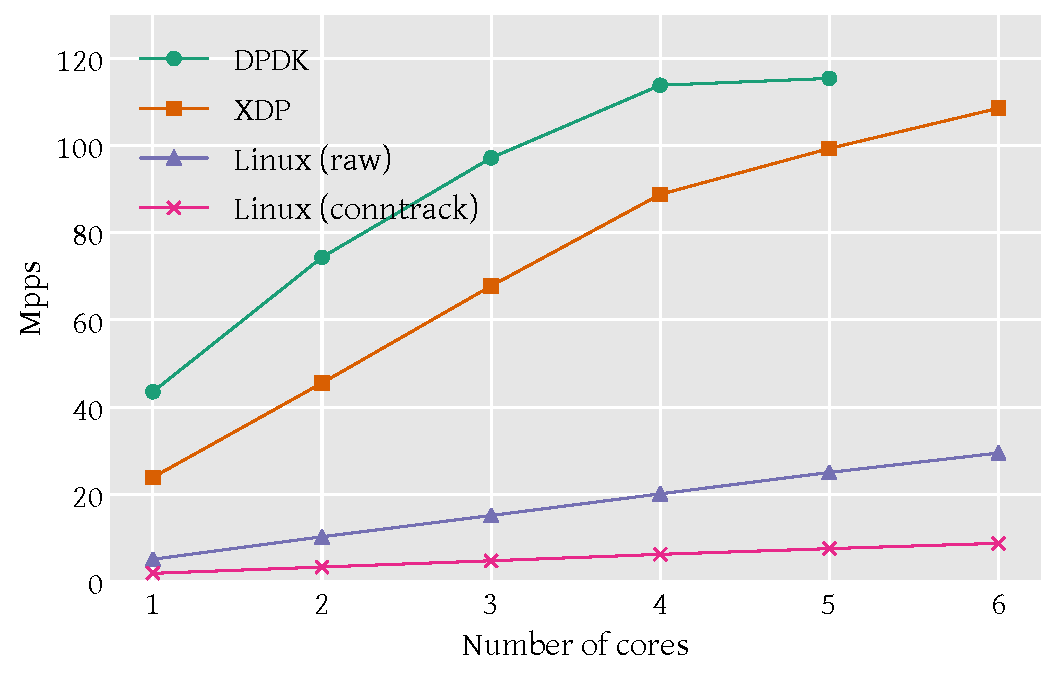
\includegraphics[width=0.95\textwidth,height=5.5cm]{original/drop-test.pdf} % first figure itself
        \subcaption{Packet drop performance in Higher PPS}
        \label{graph:xdp-drop:a}
    \end{minipage}\hfill
    \begin{minipage}{0.49\textwidth}
        \centering
        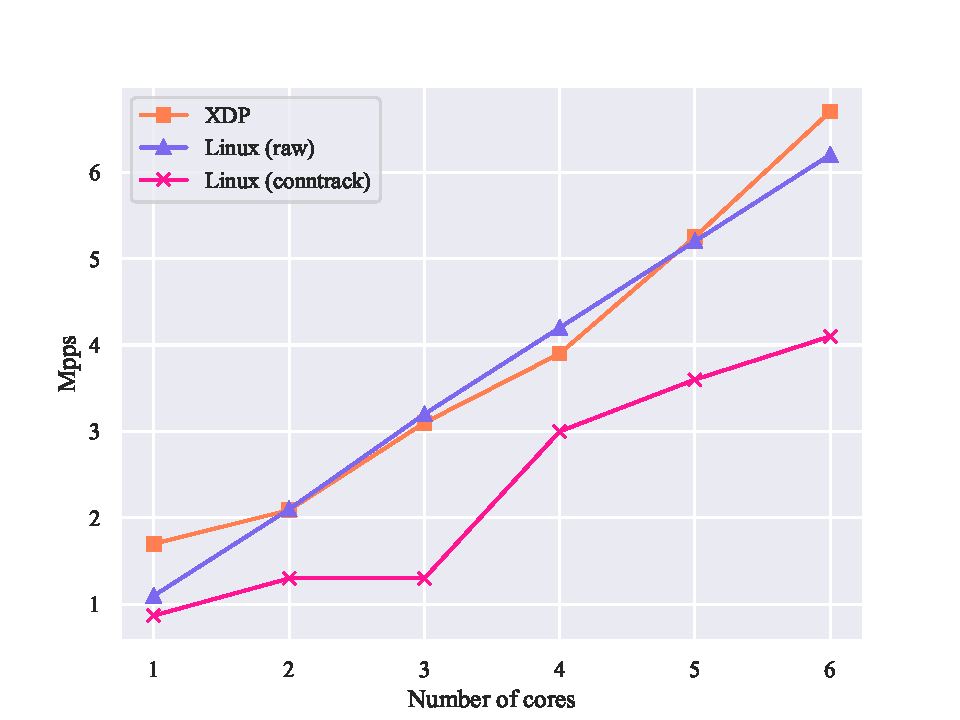
\includegraphics[width=0.95\textwidth,height=5.5cm]{img/drop-test.pdf} % second figure itself
        \subcaption{Packet drop performance in Lower PPS.}
        \label{graph:xdp-drop:b}
    \end{minipage}
     \caption{Packet drop performance.}
     \label{graph:xdp-drop}
\end{figure}

For example, Figure~\ref{graph:xdp-drop:b} compares the performance of XDP and Linux

\subsection{CPU Usage}

\begin{figure}
    \centering
    \begin{minipage}{0.49\textwidth}
        \centering
        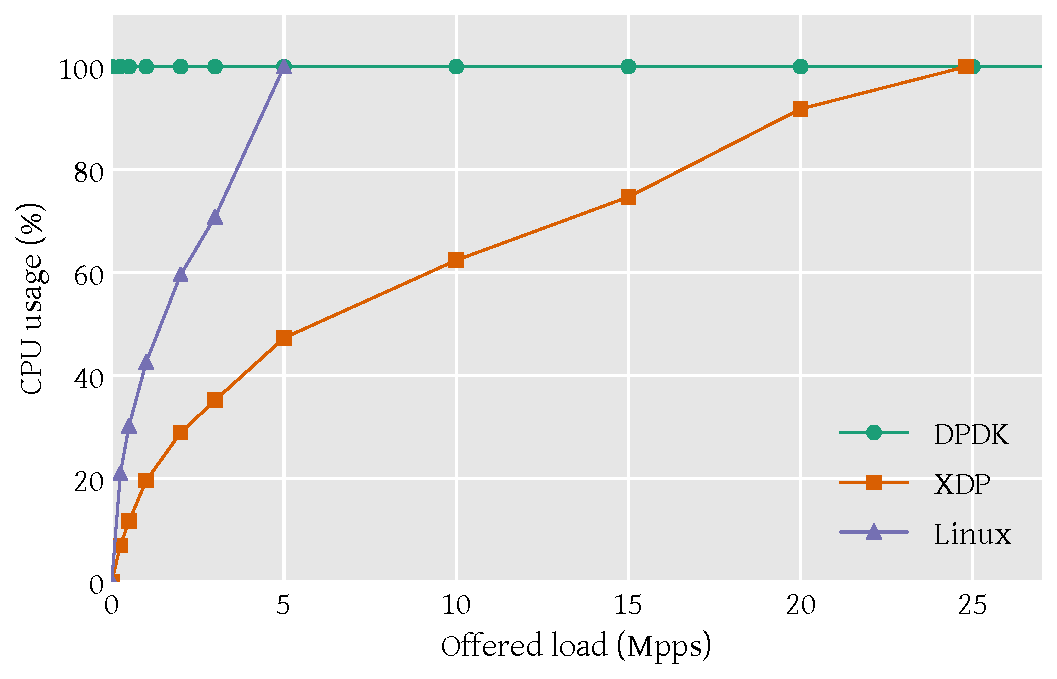
\includegraphics[width=0.95\textwidth,height=5.5cm]{original/drop-cpu.pdf} % first figure itself
        \subcaption{CPU usage in Higher PPS}
        \label{graph:drop-cpu:a}
    \end{minipage}\hfill
    \begin{minipage}{0.49\textwidth}
        \centering
        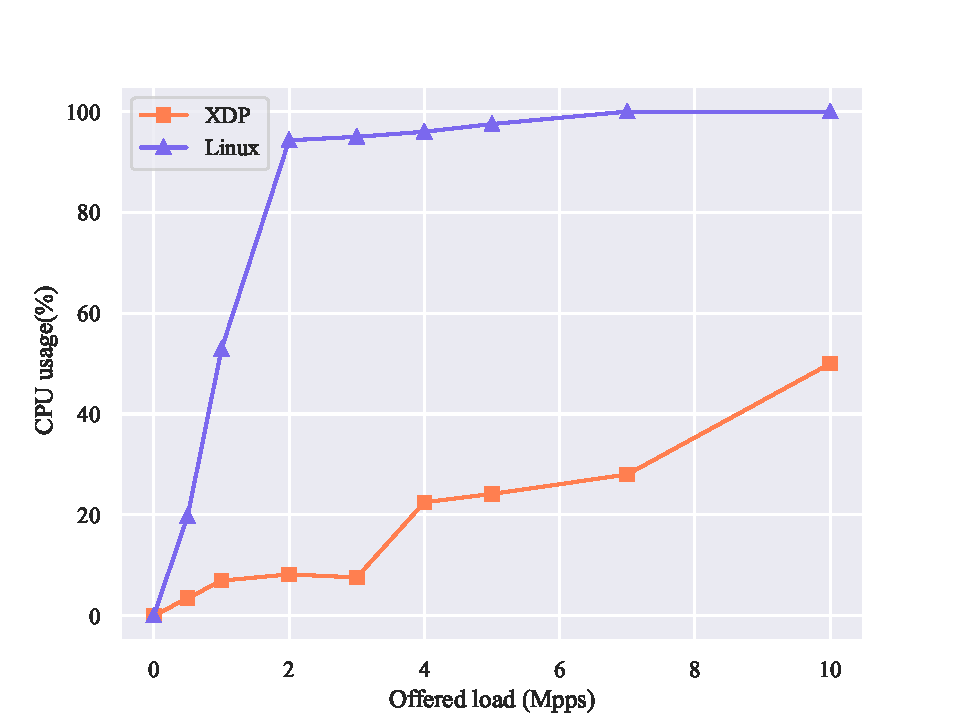
\includegraphics[width=0.95\textwidth,height=5.5cm]{img/drop-cpu.pdf} % second figure itself
        \subcaption{CPU usage in Lower PPS.}
        \label{graph:drop-cpu:b}
    \end{minipage}
     \caption{CPU usage in the drop scenario.}
     \label{graph:drop-cpu}
\end{figure}

For example, Figure~\ref{graph:drop-cpu:b} compares the performance of XDP and Linux


\subsection{Packet Forwarding Performance}

\begin{figure}
    \centering
    \begin{minipage}{0.49\textwidth}
        \centering
        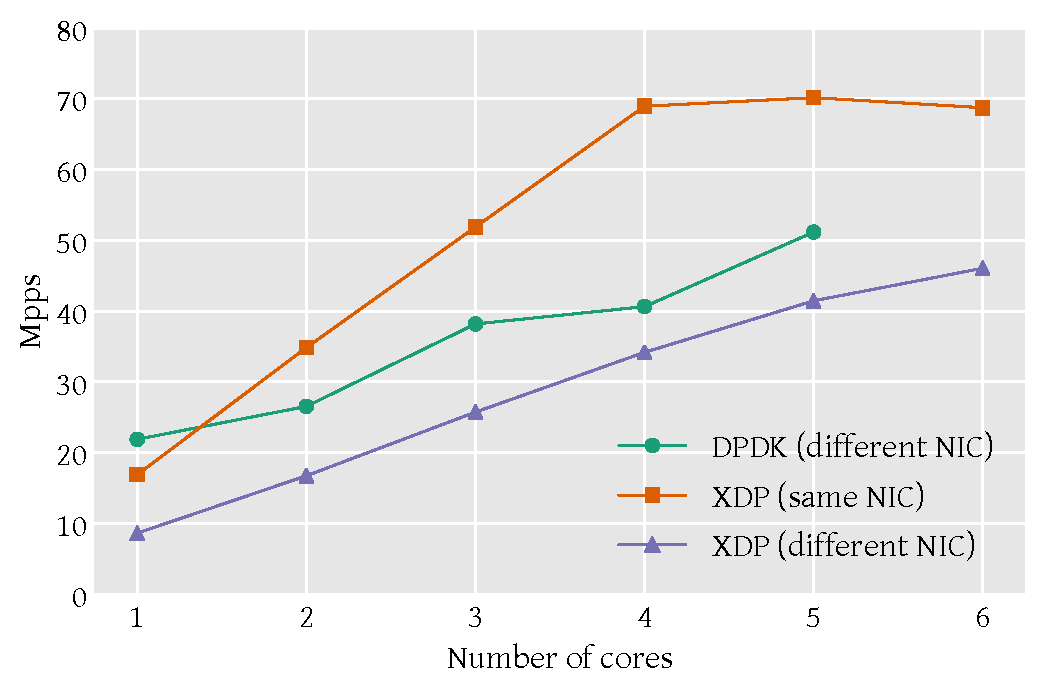
\includegraphics[width=0.95\textwidth,height=5.5cm]{original/redirect-test.pdf} % first figure itself
        \subcaption{throughput in Higher PPS}
        \label{graph:redirect:a}
    \end{minipage}\hfill
    \begin{minipage}{0.49\textwidth}
        \centering
        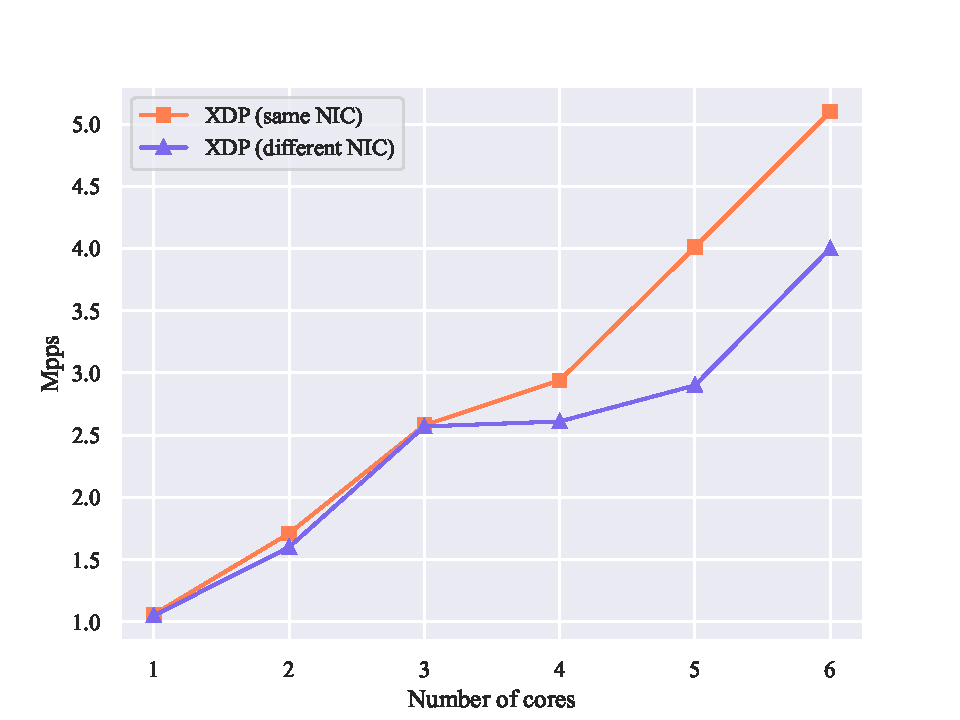
\includegraphics[width=0.95\textwidth,height=5.5cm]{img/redirect-test.pdf} % second figure itself
        \subcaption{throughput in Lower PPS.}
        \label{graph:redirect:b}
    \end{minipage}
     \caption{Packet forwarding throughput}
     \label{graph:redirect}
\end{figure}

For example, Figure~\ref{graph:redirect:b} compares the performance of XDP and Linux


\section{Real-world use cases}

\subsection{Software Routing}

\subsection{Inline DoS Mitigation}

\begin{figure}
    \centering
    \begin{minipage}{0.49\textwidth}
        \centering
        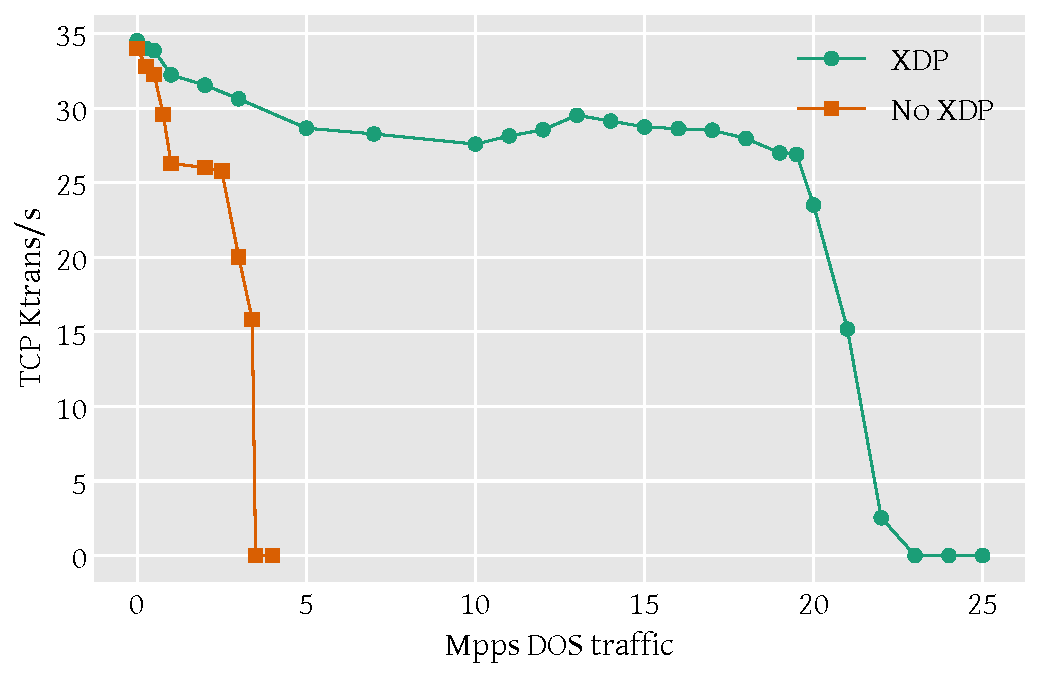
\includegraphics[width=0.95\textwidth,height=5.5cm]{original/ddos-test.pdf} % first figure itself
        \subcaption{throughput in Higher PPS}
        \label{graph:ddos:a}
    \end{minipage}\hfill
    \begin{minipage}{0.49\textwidth}
        \centering
        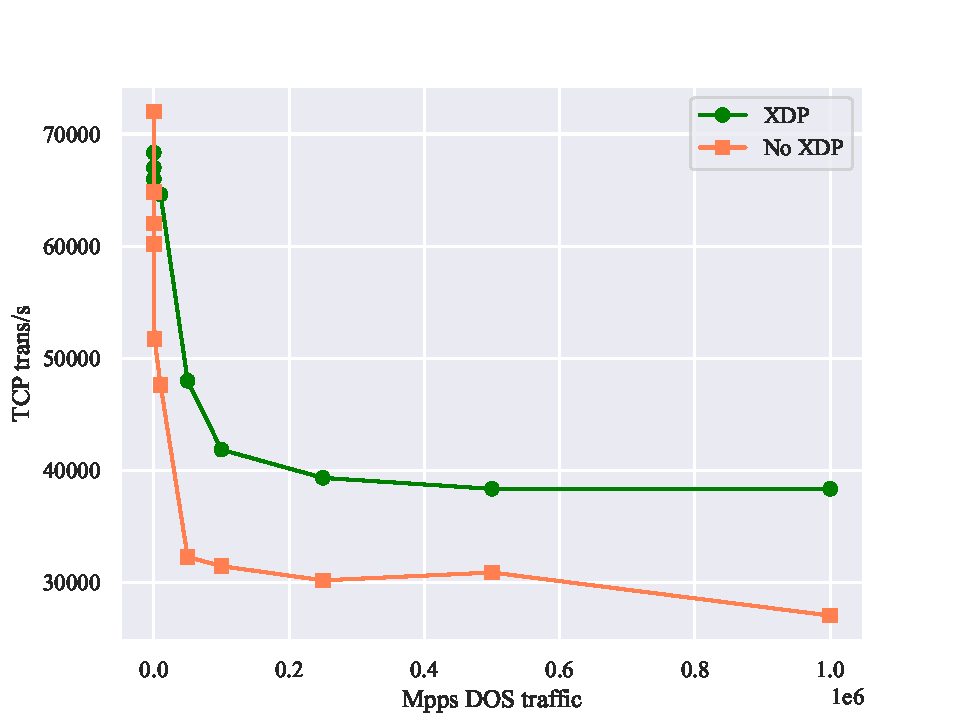
\includegraphics[width=0.95\textwidth,height=5.5cm]{img/dos-test.pdf} % second figure itself
        \subcaption{throughput in Lower PPS.}
        \label{graph:ddos:b}
    \end{minipage}
     \caption{DDoS performance. Number of TCP transactions per second as the level of attack traffic directed at the server increases}
     \label{graph:ddos}
\end{figure}

For example, Figure~\ref{graph:ddos:b} compares the performance of XDP and Linux


\section{Conclusion}

XDP is faster


%%%%%%%%%%%%%%%%%%%%%%%%
% Bibliography Begins Here %
%%%%%%%%%%%%%%%%%%%%%%%%


\begin{spacing}{1}
\bibliographystyle{plainnat}
\bibliography{xdp_report}
\end{spacing}

\end{document}
